\documentclass[class=ctexart,crop=false]{standalone}

\usepackage{amsmath,amssymb,enumitem,empheq,tkz-euclide,
diagbox,wrapfig,pgfplots}
\pgfplotsset{compat=newest}
\renewcommand\parallel{\mathrel{/\mskip-2.5mu/}}

\newcommand\px{\mathrel{/\mkern-5mu/}}  %平行
\newcommand\pxeq{\mathrel{\vcenter{     %平行且等于
\ialign{\hfil##\hfil\crcr
$\scriptstyle\px\!$\crcr
\noalign{\nointerlineskip\vskip1pt}$=$\crcr}}}}

%\setCJKmainfont{SimSun}       %设置西文字体为times new roman
%\setCJKsansfont{SimSun}             %设置中文字体为宋体
%\setCJKmonofont{STKaiti}
%\setsansfont{TeX Gyre Termes}            %设置typewriter family中文字体为楷体
%\setmonofont{TeX Gyre Termes}

\usetikzlibrary{calc,intersections,through,backgrounds,patterns}
\newcounter{para}
\newcommand\mypara{\par\refstepcounter{para}\thepara.\space}%设置typewriter family西文字体为times new roman
\newcommand*\circled[1]{\tikz[baseline=(char.base)]{
            \node[shape=circle,draw,inner sep=1.3pt] (char) {#1};}}
\begin{document}
如图,在长方体 $ABCD-A_1B_1C_1D_1$中,点 $D,E$ 分别在棱 $DD_1,BB_1$上,且
$2DE=ED_1,BF=2FB_1.\\$
\begin{wrapfigure}{r}{0.3\textwidth}
    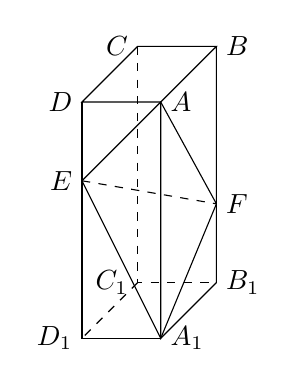
\begin{tikzpicture}[scale=1]
            \coordinate[label=right:$A_1$] (A_1) at (0,0);
            \coordinate[label=right:$A$] (A) at (0,3);
            \coordinate[label=right:$B_1$] (B_1) at ($sqrt(2)*(0.5,0.5)$);
            \coordinate[label=right:$B$] (B) at ($sqrt(2)*(0.5,0.5)+(0,3)$);
            \coordinate[label=left:$C_1$] (C_1) at ($sqrt(2)*(0.5,0.5)+(-1,0)$);
            \coordinate[label=left:$C$] (C) at ($sqrt(2)*(0.5,0.5)+(-1,3)$);
            \coordinate[label=left:$D_1$] (D_1) at (-1,0);
            \coordinate[label=left:$D$] (D) at (-1,3);
            \coordinate[label=left:$E$] (E) at (-1,2);
            \coordinate[label=right:$F$] (F) at ($sqrt(2)*(0.5,0.5)+(0,1)$);
            \draw (A)--(B)--(C)--(D)--(A)--(A_1)--(B_1)--(B);
            \draw (A_1)--(D_1)--(D);
            \draw[dashed] (C)--(C_1)--(B_1);
            \draw[dashed] (C_1)--(D_1);
            \draw (E)--(A)--(F);
            \draw (E)--(A_1)--(F);
            \draw[dashed] (E)--(F);
    \end{tikzpicture}
\end{wrapfigure}

\begin{enumerate}[label=(\arabic*)]
    \item 证明:点 $C_1$ 在平面 $AEF$ 内;
    \item 若 $AB=2,AD=1,AA_1=3,$求二面角 $A-EF-A_1$的正弦值.
\end{enumerate}


\end{document}